\documentclass[11pt]{article}
\usepackage{textcomp}

\RequirePackage[USenglish]{babel}
\RequirePackage{microtype}          % Better typography
\usepackage{pacioli}
\RequirePackage[OT1]{fontenc}        %
\RequirePackage[utf8]{inputenc}     %
\RequirePackage{fancyhdr}           %
\RequirePackage{geometry}           %
\RequirePackage{lmodern}            %
\RequirePackage{amsmath}            % /*
\RequirePackage{amsfonts}           %    The math packages
\RequirePackage{amssymb}            % */
\RequirePackage{csquotes}           % Nice quotes
\RequirePackage[svgnames]{xcolor}   % Colors!
\RequirePackage{graphicx}           %
\RequirePackage{parskip}
\RequirePackage{subfiles}
\RequirePackage{pgfornament}        % Ornaments
\RequirePackage{background}         % in the background!
\RequirePackage{booktabs}
\RequirePackage{pgffor}
\RequirePackage{hyperref}           % Make the links colorful!

\geometry{a4paper, total={17cm,24cm}}


\pagestyle{fancy}
\fancyhf{}
\def\currentCategoryName{}

\fancyfoot[c]{\\[10pt]\Large\thepage}
% This has to be done in this way, instead of setting \fancyhead directly, because some form of global state and variables are involved.
% This, in turn, leads to subfiles not being able to set the header for the main file. So use a \xdef to store it globally

\fancyhead[c]{\LARGE \textsc{\currentCategoryName}}
\def\category#1{%
  \xdef\currentCategoryName{#1}
}



% Make the fancy header options.
\setlength{\headheight}{30pt}
\setlength{\headsep}{20pt}
\setlength{\footskip}{20pt}
\renewcommand{\headrulewidth}{0.5pt}
\renewcommand{\footrulewidth}{0.5pt}
\def\theHeadRuleWidth{0.85}

\setlength{\tabcolsep}{5pt}  % More space in tables.
\setlength{\parindent}{0pt}  % No indents on newline.

% 15
\def\cornerOrnament{63}
\def\categoryOrnament{79}
\def\theWidth{110pt}
\backgroundsetup{
    scale=1,
    opacity=1,
    angle=0,
    color=black,
    contents={%
        \begin{tikzpicture}[every node/.style={inner sep=0pt}]
            \node[anchor=north west](CNW)
            at (current page.north west) {\pgfornament[width=\theWidth]{\cornerOrnament}};
            \node[anchor=north east](CNE)
            at (current page.north east) {\pgfornament[width=\theWidth,symmetry=v]{\cornerOrnament}};
            \node[anchor=south west](CSW)
            at (current page.south west) {\pgfornament[width=\theWidth,symmetry=h]{\cornerOrnament}};
            \node[anchor=south east](CSE)
            at (current page.south east) {\pgfornament[width=\theWidth,symmetry=c]{\cornerOrnament}};
            %
            \node[anchor=north west, xshift=3.7cm, yshift=-0.3cm](CNE)
            at (current page.north west) {\pgfornament[scale=0.37]{\categoryOrnament}};
            \node[anchor=north east, xshift=-3.7cm, yshift=-0.3cm](CNE)
            at (current page.north east) {\pgfornament[symmetry=v, scale=0.37]{\categoryOrnament}};
            %
        \end{tikzpicture}%
    }
}

\renewcommand\headrule{\makebox[\textwidth]{\rule{\theHeadRuleWidth\headwidth}{\headrulewidth}} \vskip-\headrulewidth}
\renewcommand\footrule{\makebox[\textwidth]{\rule{\theHeadRuleWidth\headwidth}{\footrulewidth}} \vskip-\footrulewidth}


\date{}


% TODO: Add a feature to print in oz / ml
\def\ml#1{%
    \pgfmathsetmacro\result{#1 * 0.0333}%0.03814}%
    \pgfmathprintnumberto[precision=2]{\result}{\result}%
    #1 ml% (\result~oz.)%
}
\def\counter{1}
\def\cocktailDivider{\rule{\textwidth}{0.5pt}}

\def \ifempty#1{\def\temp{#1} \ifx\temp\empty }
% #1 = name, #2 = ingredients (pgffor), #3 = Equipment (pgffor), #4 = Method (pgffor)
\def\cocktail#1#2#3#4{
    \smallskip
    \begin{center}
    {\Large\bf#1}
    \end{center}
    \medskip
    %
    \fontsize{12}{16}\selectfont
%    \textbf{Ingredients:}
    \begin{minipage}[t]{0.49\textwidth}%
        \vspace{0pt}
        \begin{itemize}
            \foreach \x in {#2} {%
                \item \x
            }
        \end{itemize}
    \end{minipage}
    %
    \begin{minipage}[t]{0.49\textwidth}%
        \vspace{0pt}
        \begin{enumerate}
            \foreach \x in {#4} {%
                \item \x
            }
        \end{enumerate}
    \end{minipage}

    \ifempty{#3}
    \else
    \medskip
    \begin{center}
        \textsl{Tools: \foreach[count=\i] \x in {#3}{%
            \ifnum%
            \i=1\else%
            , %
            \fi\x}}%
    \end{center}
    \fi
}

\begin{document}

\subfile{cocktail-categories/classics.tex}
\clearpage

\subfile{cocktail-categories/serene-spirits.tex}
\clearpage

\subfile{cocktail-categories/tropical-vibes.tex}
\clearpage

\subfile{cocktail-categories/fresh-and-fruity.tex}



%
%\cocktail{Mojito}{
%    \ml{60} White rum,
%    \ml{20} Fresh lime juice,
%    \ml{20} Sugar syrup,
%    6 -- 8 Mint leaves,
%    Top soda water (optional),
%    Crushed ice,
%    Mint sprig to garnish
%}
%%
%{jigger, barspoon, highball glass, tea towel, wooden mallet/rolling pin, bar
%napkin (unless you’re making it for yourself!)}
%%
%{
%    {Crush your ice if you don’t have a crushed ice machine to hand. Use tea towel and
%    wooden mallet for this (wrap ice in tea towel, then smash).},
%    Add all ingredients to glass and fill with ice to just under top of glass.,
%    {    I don’t muddle -- just give the mint a gentle clap -- so as to keep the drink
%    lighter and fresher, but if you do, do it gently.},
%    Place barspoon in the glass and cover the top with the bar napkin.,
%    {Churn through, add more ice and repeat until the glass is pretty much full and the
%    mint is suspended through the drink.},
%    Top with a cap of crushed ice and some soda water if you like a little spritz.,
%    {Garnish with a mint sprig, and enjoy!}
%}
%
%
%
%\cocktail{Long Island Ice Tea}{
%    \ml{15} Vodka,
%    \ml{15} Gin,
%    \ml{15} White rum,
%    \ml{15} Tequila,
%    \ml{15} Curacao/triple sec,
%    \ml{15} Sugar syrup,
%    \ml{30} Fresh lemon juice,
%    Around \ml{45} Coca Cola,
%    A skewered lemon wheel and cocktail cherry to garnish
%}
%%
%{jigger, shaker tins, hawthorn strainer, highball glass}
%%
%{
%    Add all of your ingredients except your coca cola to your shaker tins.,
%    Pour the coca cola in to your serving glass.,
%    {Fill your shaker tin with ice, seal and shake hard.},
%    {Pop the tins open, but before you pour, add ice to your serving glass.},
%    Use hawthorn strainer to hold the ice back in your tins and pour slowly over fresh
%    ice -- this should create a layered effect.,
%    {Garnish with your skewered lemon and cherry, and enjoy!}
%}



%\cocktail{ZOMBIE}{
%    \ml{25} Dark Rum,
%    \ml{25} Golden Rum,
%    \ml{25} Triple Sec,
%    \ml{15} Lime Juice,
%    \ml{40} Orange Juice,
%    \ml{25} Passionfruit Puree,
%    \ml{7.5} Grenadine,
%    2 Dashes Angostura Bitter
%}
%%
%{jigger, shaker tins, rocks glass, straw}
%%
%{
%    Add all ingredients to a cocktail shaker.,
%    Add ice to the mix and then shake well for around 30 seconds.,
%    Strain using a hawthorn strainer into a Collins or Hi-Ball glass.,
%    Garnish with mint sprig \& orange slice.
%}
%

%
%\cocktail{London Calling}{
%    \ml{40} London Dry gin (Navy Strength if you can find it),
%    \ml{15} Fresh lemon juice,
%    \ml{15} Fino sherry,
%    \ml{15} Sugar syrup,
%    2 Dashes of orange bitters,
%    Good ice,
%    Grapefruit twist to garnish
%}
%%
%{coupe, jigger, shaker tins, hawthorn strainer, fine strainer}
%%
%{
%    Add all of the ingredients to your shaker tin.,
%    Fill shaker tin full with ice. Combine tins and shake hard until the tins get frosted.,
%    Open tins and double strain (use the hawthorn strainer to hold the ice back in the tin and pour through the fine strainer) into a chilled coupe.,
%    Squeeze the grapefruit twist to expel the citrus oil over the drink then add the twist to the drink.
%}

%    \cocktail{1934 Cosmopolitan Cocktail}{
%        \ml{60} Gin,
%        \ml{15} Cointreau,
%        \ml{25} Lemon Juice,
%        \ml{10} Raspberry Syrup,
%        2 dashes of orange bitters
%    }
%%
%    {jigger, shaker tins, fine strainer, chilled coupe glass}
%%
%    {
%        Shake all ingredients with ice.,
%        Fine strain into chilled coupe glass.
%    }


%\cocktail{Sazerac}{
%    \ml{60} Rye,
%    \ml{10} Sugar syrup,
%    10 -- \ml{15} Absinthe to rinse,
%    4 Dashes Peychaud’s bitters,
%    Lemon twist to garnish
%}
%%
%{jigger, mixing glass, barspoon, julep strainer, small rock glass, shot glass}
%%
%{
%    {Prepare a small coin of lemon peel.},
%    {Fill serving glass with ice, add the absinthe, give a stir and leave to chill.},
%    {Add all of the other ingredients to your mixing glass.},
%    {Fill with ice, stir by pushing the ice around with the back of your spoon against the inside of the glass.},
%    {Once chilled and diluted, strain the absinthe from the serving glass into the shot glass and discard the ice, then strain the drink into the serving glass.},
%    {Fold your lemon peel sharply over the drink to expel the oils, then discard.},
%    {Serve your Sazerac with the absinthe on the side (if you like!).}
%}
%
%
%\cocktail{Hemingway Daiquiri}{
%    \ml{60} White rum,
%    \ml{15} Lime juice,
%    \ml{15} Grapefruit juice,
%    \ml{10} Maraschino liqueur,
%    \ml{5} Sugar syrup,
%    Maraschino cherry to garnish,
%    Grapefruit zest to twist and discard
%}
%%
%{shaker tins, jigger, hawthorne strainer, fine strainer, straw for tasting}
%%
%{
%    {Add all non-garnish ingredients to shaker tins with ice.},
%    {Shake hard until the tins get frosted.},
%    {Taste test with straw (grapefruit is sometimes quite bitter depending on the season).},
%    {Double strain into chilled coupe glass.},
%    {Twist grapefruit zest over drink, then discard.},
%    {Pop maraschino cherry into drink as garnish.}
%}
%
%\cocktail{Final Ward}{
%    \ml{22.5} Rye whiskey,
%    \ml{22.5} Green Charteuse,
%    \ml{22.5} Maraschino,
%    \ml{22.5} Lemon juice,
%    Optional: Maraschino cherry to garnish
%}
%%
%{jigger, shaker tins, fine strainer, chilled coupe glass}
%%
%{
%    Combine all ingredients in a cocktail shaker.,
%    Shake with ice and strain into a coupe glass.,
%    (Optional) Garnish with Maraschino cherry
%}
%


% TODO: Add Green Mamba

\end{document}
